

\chapter{VBF Tag \Zee Validation Plots}
\label{appendix:vbf_zee}



\begin{figure}[h!]
    \begin{center}
        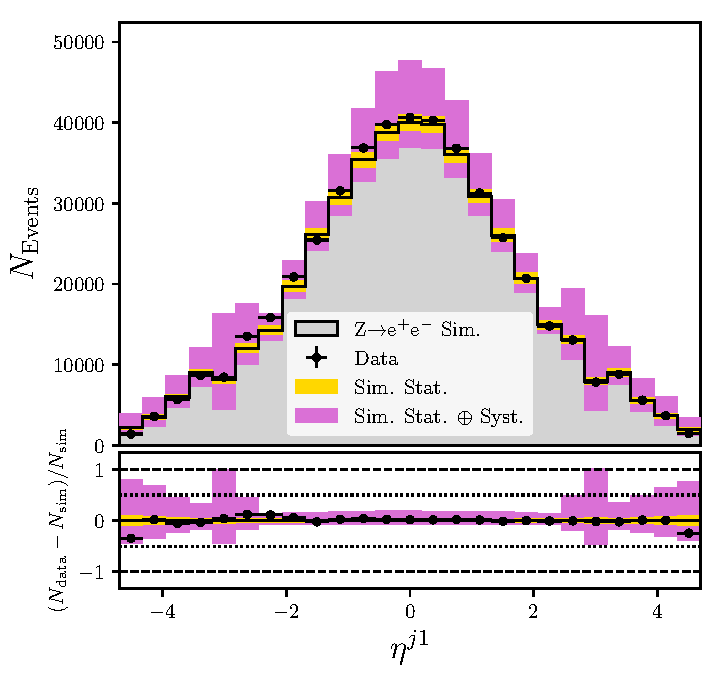
\includegraphics[width=0.49\textwidth]{figures/appendix_zee/lead_jet_eta_zee_LPS.pdf}
        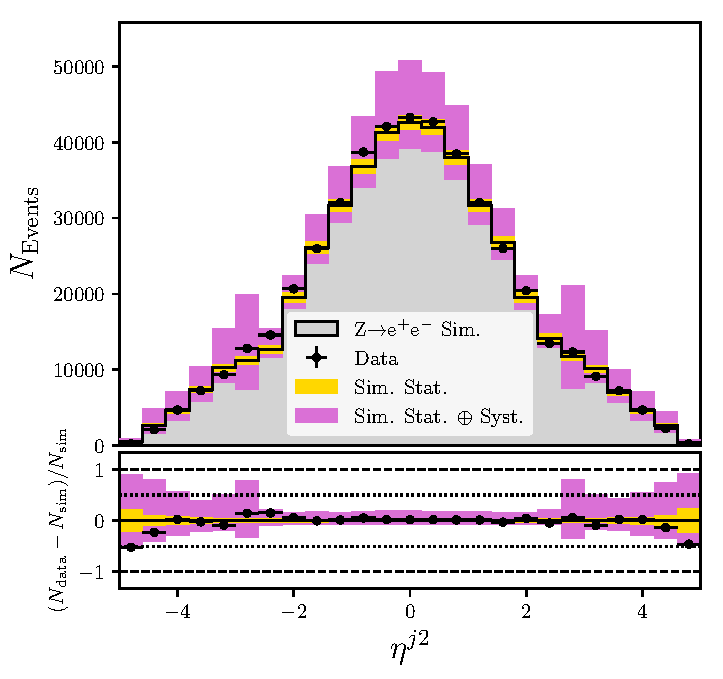
\includegraphics[width=0.49\textwidth]{figures/appendix_zee/sublead_jet_eta_zee_LPS.pdf}
    \end{center}
    \caption{\Zee validation plots of pseudorapidity distributions for leading jet in $p_T$ (left) and subleading jet (right).}
\end{figure}

\begin{figure}[h!]
    \begin{center}
        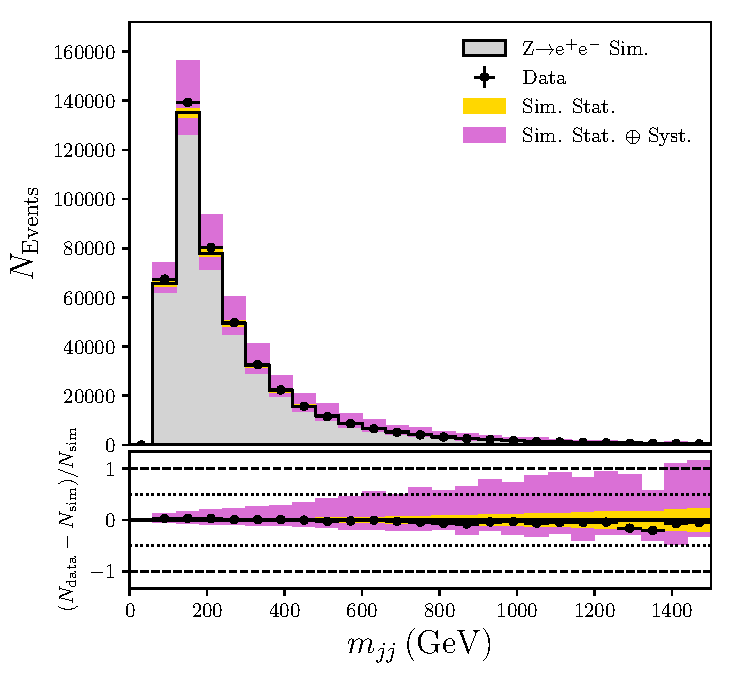
\includegraphics[width=0.49\textwidth]{figures/appendix_zee/dijet_mass_zee_LPS.pdf}
        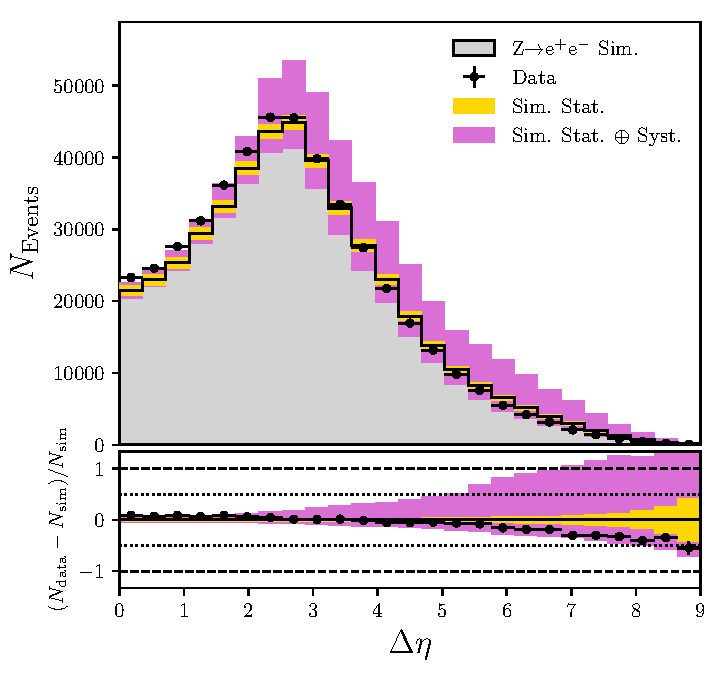
\includegraphics[width=0.49\textwidth]{figures/appendix_zee/delta_eta_zee_LPS.pdf}
    \end{center}
    \begin{center}
        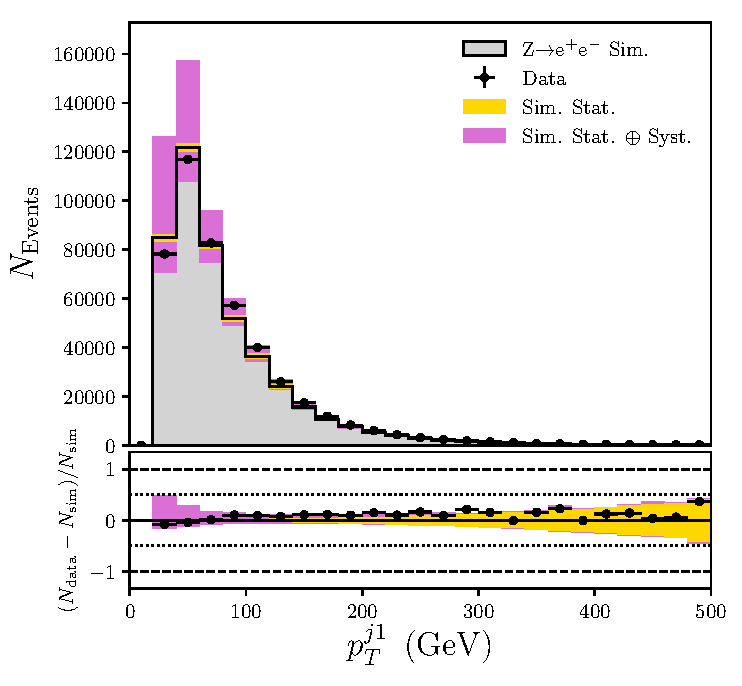
\includegraphics[width=0.49\textwidth]{figures/appendix_zee/lead_jet_pt_zee_LPS.pdf}
        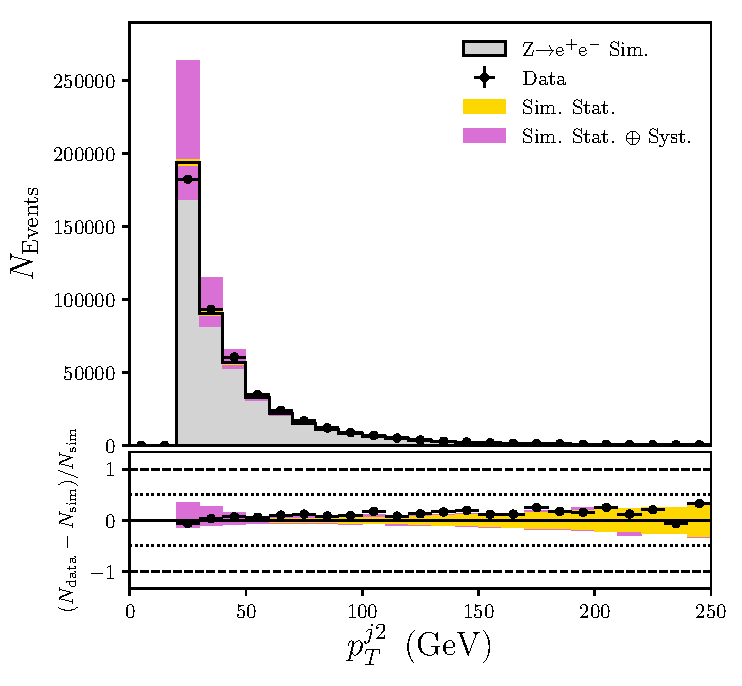
\includegraphics[width=0.49\textwidth]{figures/appendix_zee/sublead_jet_pt_zee_LPS.pdf}
    \end{center}
    \begin{center}
        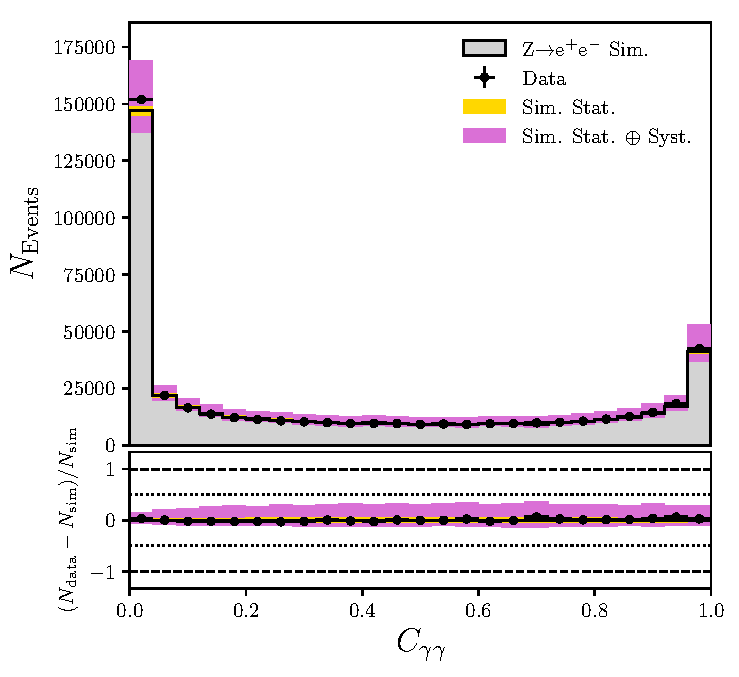
\includegraphics[width=0.49\textwidth]{figures/appendix_zee/centrality_zee_LPS.pdf}
        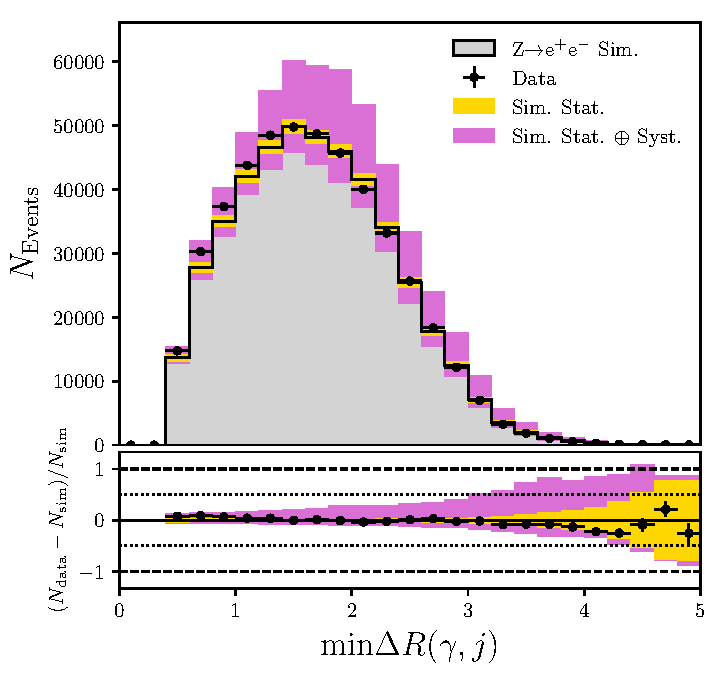
\includegraphics[width=0.49\textwidth]{figures/appendix_zee/min_delta_r_jgam_zee_LPS.pdf}
    \end{center}
    \caption{\Zee validation plots for kinematic features used by the VBF tag. Clockwise from top left: dijet mass, dijet pseudorapidity gap, subleading jet \pt, 
             minimum $\Delta{R}$ between either photon and either jet, centrality, and leading jet \pt.}
\end{figure}

\begin{figure}[h!]
    \begin{center}
        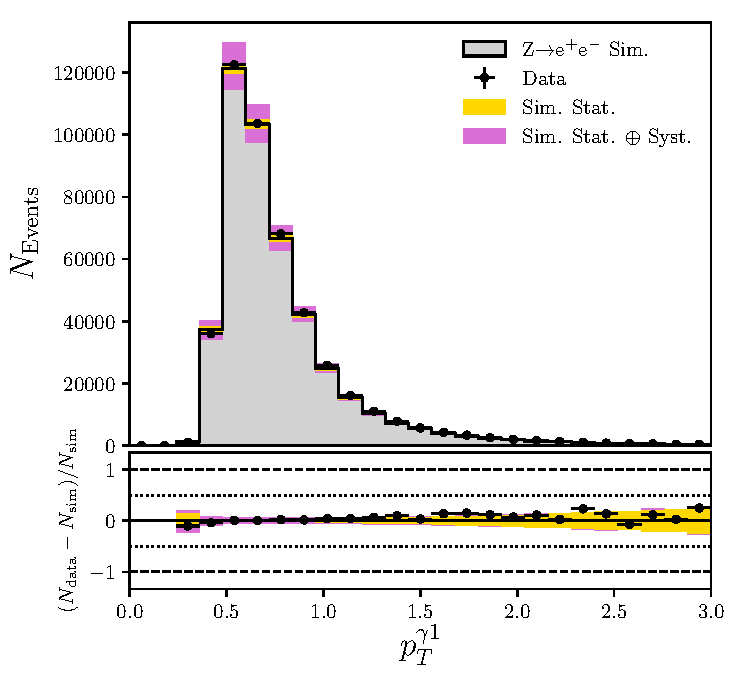
\includegraphics[width=0.49\textwidth]{figures/appendix_zee/lead_ptom_zee_LPS.pdf}
        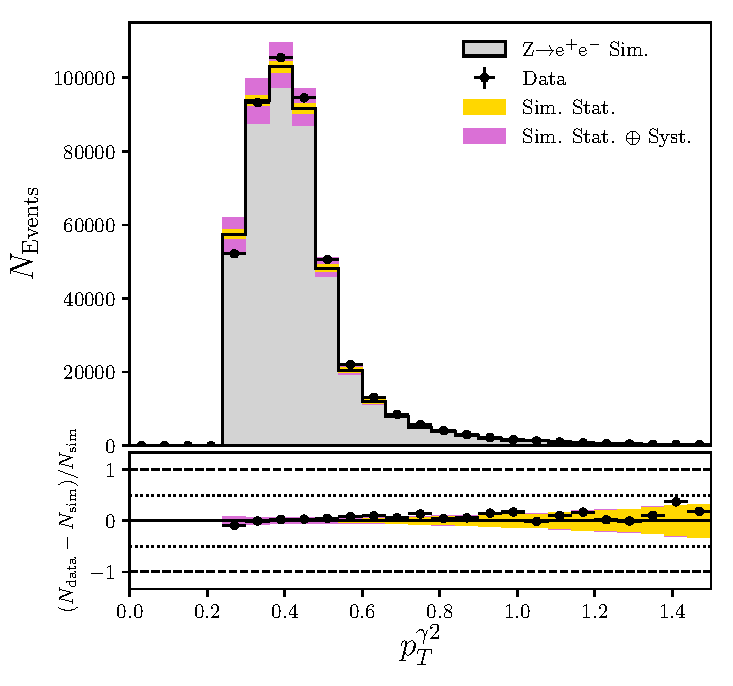
\includegraphics[width=0.49\textwidth]{figures/appendix_zee/sublead_ptom_zee_LPS.pdf}
    \end{center}
    \begin{center}
        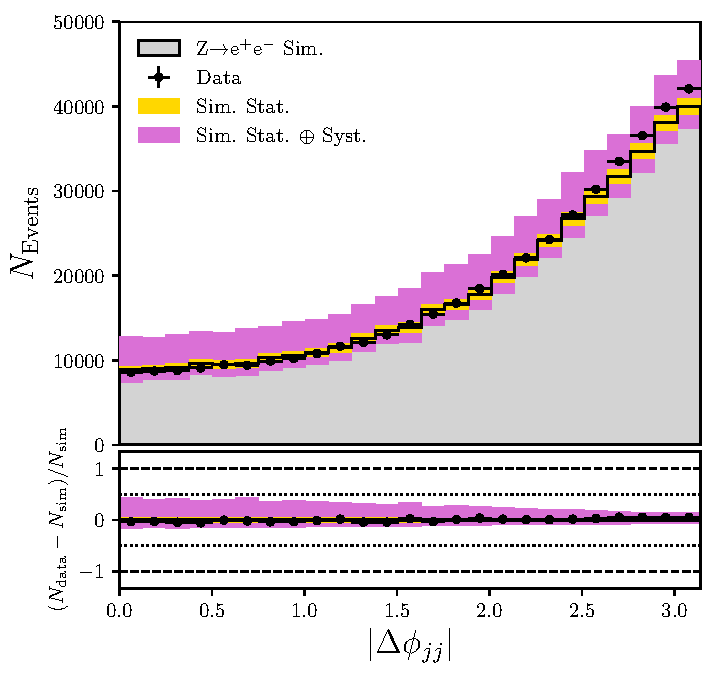
\includegraphics[width=0.49\textwidth]{figures/appendix_zee/dphi_jetjet_zee_LPS.pdf}
        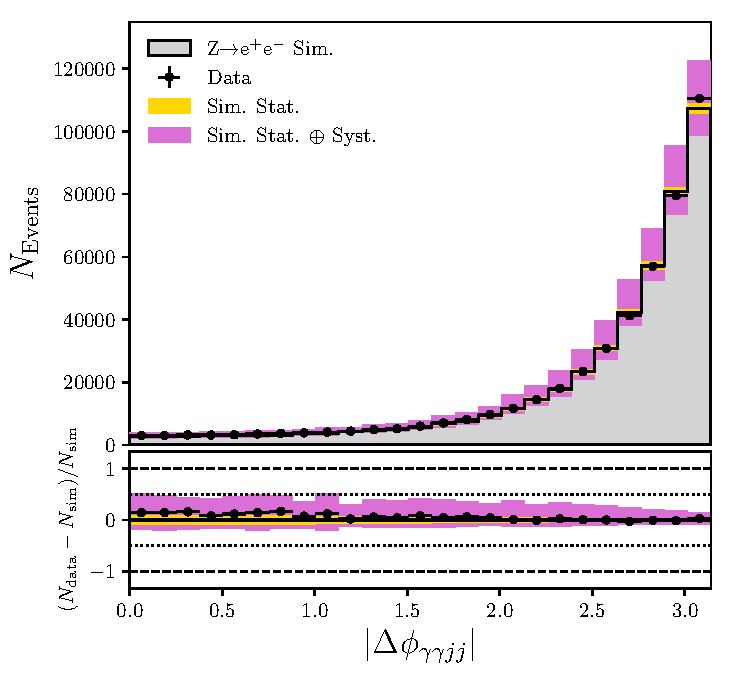
\includegraphics[width=0.49\textwidth]{figures/appendix_zee/dphi_gamgamjetjet_zee_LPS.pdf}
    \end{center}
    \begin{center}
        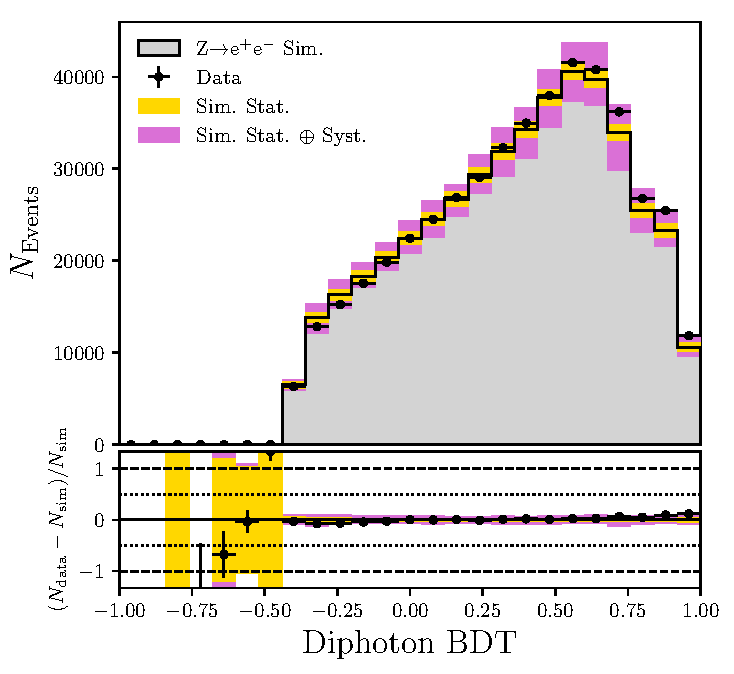
\includegraphics[width=0.49\textwidth]{figures/appendix_zee/dipho_bdt_zee_LPS.pdf}
        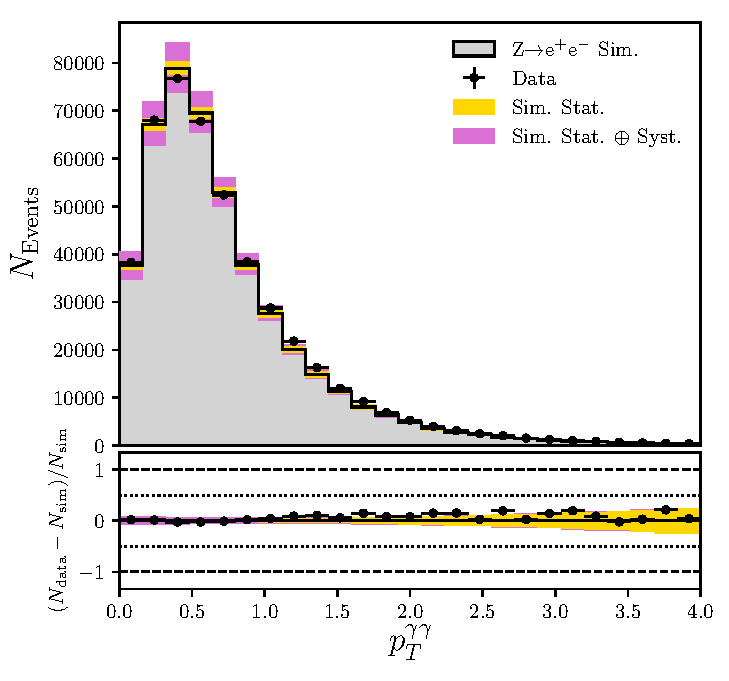
\includegraphics[width=0.49\textwidth]{figures/appendix_zee/total_ptom_zee_LPS.pdf}
    \end{center}
    \caption{\Zee validation plots for kinematic features used by the VBF tag. Clockwise from top left: leading photon \pt scaled by the diphoton mass, 
             subleading photon \pt scaled by the diphoton mass, azimuthal angular difference between dijet and diphoton, total diphoton \pt scaled by diphoton mass,
             diphoton BDT score, and azimuthal angular difference between the dijet jets.}
\end{figure}


